\section{}
% The streamwise velocity component of a steady, incompressible, laminar, flat 
% plate boundary layer of boundary layer thickness 𝛿 is approximated by the simple 
% linear expression, 𝑢 = 𝑈𝑦/𝛿 for 𝑦 < 𝛿, and 𝑢 = 𝑈 for 𝑦 > 𝛿 (see Figure 2). 
% Generate expressions for displacement thickness and momentum thickness as 
% functions of 𝛿, based on this linear approximation. Compare the approximate 
% values of 𝛿
% ∗
% /𝛿 and 𝜃/𝛿 to the values of 𝛿
% ∗
% /𝛿 and 𝜃/𝛿 obtained from the Blasius 
% solution.

\textit{The streamwise velocity component of a steady, incompressible, laminar, flat plate boundary layer of boundary layer thickness $\delta$ is approximated by the simple linear expression, $u = Uy/\delta$ for $y < \delta$, and $u = U$ for $y > \delta$ (see Figure \ref{fig:q3_flat_plate}). Generate expressions for displacement thickness and momentum thickness as functions of $\delta$, based on this linear approximation. Compare the approximate values of $\delta^*/\delta$ and $\theta/\delta$ to the values of $\delta^*/\delta$ and $\theta/\delta$ obtained from the Blasius solution.}
\begin{figure}[H]
    \centering
    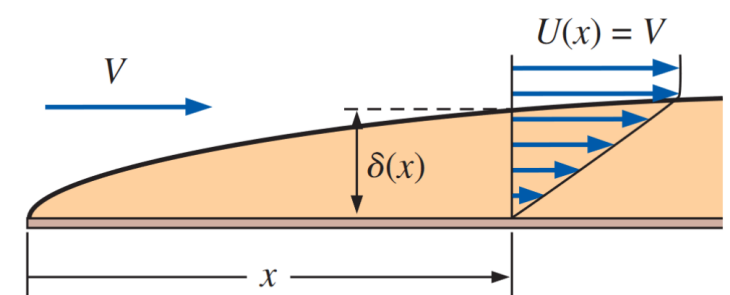
\includegraphics[width=0.5\textwidth]{Questions/Figures/Q3 Problem Diagram.png}
    \caption{Flat Plate Boundary Layer}
    \label{fig:q3_flat_plate}
\end{figure}

By conservation of mass, 
\begin{align*}
    \delta^* &= \int_{0}^{\delta} \left( 1 - \frac{y}{\delta} \right) dy \\
    &= \left[ y - \frac{y^2}{2\delta} \right]_{0}^{\delta} \\
    &= \delta - \frac{\delta^2}{2\delta} \\
    &= \frac{\delta}{2}
\end{align*}
or more conveniently,
\begin{align*}
    \Aboxed{\frac{\delta^*}{\delta} &= \frac{1}{2}}
\end{align*}
By conservation of momentum,
\begin{align*}
    \theta &= \int_{0}^{\delta} \frac{u}{U} \left( 1 - \frac{u}{U} \right) dy \\
    &= \int_{0}^{\delta} \frac{y}{\delta} \left( 1 - \frac{y}{\delta} \right) dy \\
    &= \int_{0}^{\delta} \left( \frac{y}{\delta} - \frac{y^2}{\delta^2} \right) dy \\
    &= \left[ \frac{y^2}{2\delta} - \frac{y^3}{3\delta^2} \right]_{0}^{\delta} \\
    &= \frac{\delta^2}{2\delta} - \frac{\delta^3}{3\delta^2} \\
    &= \frac{\delta}{2} - \frac{\delta}{3} \\
    &= \frac{\delta}{6}
\end{align*}
or more conveniently,
\begin{align*}
    \Aboxed{\frac{\theta}{\delta} &= \frac{1}{6}}
\end{align*}
Recall from the Blasius solution for laminar boundary layers on a flat plate,
\begin{align*}
    \frac{\delta}{x} &= \frac{4.91}{\sqrt{\text{Re}_x}} \\
    \frac{\delta^*}{x} &= \frac{1.72}{\sqrt{\text{Re}_x}} \\
    \frac{\theta}{x} &= \frac{0.664}{\sqrt{\text{Re}_x}}
\end{align*}
Then,
\begin{empheq}[box=\fbox]{align*}
    \frac{\delta^*}{\delta} &= \frac{1.72}{4.91} = 0.350 \\
    \frac{\theta}{\delta} &= \frac{0.664}{4.91} = 0.135
\end{empheq}
The relative errors are then,
\begin{empheq}[box=\fbox]{align*}
    \text{Error}_{\delta^*} &= \frac{0.350 - 0.5}{0.350} \times 100\% = 42.9\% \\
    \text{Error}_{\theta} &= \frac{0.135 - 0.166}{0.135} \times 100\% = 23.0\%
\end{empheq}
The approximation is not very accurate, with high errors in both $\delta^*$ and $\theta$.